\chapter{L8 -- Proprietà degli autovettori generalizzati e modi associati ai blocchi di Jordan}

\section{Obiettivo della lezione}

Nelle lezioni precedenti abbiamo introdotto:
\begin{itemize}
    \item la forma di Jordan;
    \item gli autovettori generalizzati;
    \item la costruzione delle catene associate a ciascun autovalore.
\end{itemize}

In questa lezione vogliamo chiarire tre idee fondamentali:

\begin{enumerate}
    \item quali proprietà hanno gli autovettori generalizzati;
    \item come sono collegati ai sottospazi ciclici e ai sottospazi $A$-invarianti;
    \item perché la struttura dei blocchi di Jordan determina direttamente i \emph{modi} che compaiono nell'evoluzione temporale del sistema.
\end{enumerate}

La morale della lezione è molto importante: per capire davvero l'andamento nel tempo di un sistema lineare non basta conoscere gli autovalori; bisogna conoscere anche la \emph{dimensione dei blocchi di Jordan} associati a ciascun autovalore.

\section{Richiamo: catene di autovettori generalizzati}

Sia $\lambda$ un autovalore di $A \in \R^{n\times n}$.  
Una catena di autovettori generalizzati associata a $\lambda$ è una famiglia di vettori
\[
q^{(1)}, q^{(2)}, \dots, q^{(k)}
\]
tale che
\begin{equation}
(A-\lambda I)q^{(1)} = 0,
\label{eq:L8_chain_1}
\end{equation}
\begin{equation}
(A-\lambda I)q^{(2)} = q^{(1)},
\label{eq:L8_chain_2}
\end{equation}
\[
\vdots
\]
\begin{equation}
(A-\lambda I)q^{(k)} = q^{(k-1)}.
\label{eq:L8_chain_k}
\end{equation}

Il vettore $q^{(1)}$ è un normale autovettore, mentre $q^{(j)}$ con $j\ge 2$ è un autovettore generalizzato di ordine $j$.

Equivalentemente si può scrivere:
\[
Aq^{(1)} = \lambda q^{(1)},
\]
\[
Aq^{(2)} = q^{(1)} + \lambda q^{(2)},
\]
\[
\vdots
\]
\[
Aq^{(k)} = q^{(k-1)} + \lambda q^{(k)}.
\]

\begin{figure}[H]
\centering
\begin{tikzpicture}[>=Latex, node distance=1.7cm]
    \node[draw, rounded corners] (q1) {$q^{(1)}$};
    \node[draw, rounded corners, right=of q1] (q2) {$q^{(2)}$};
    \node[right=of q2] (dots) {$\cdots$};
    \node[draw, rounded corners, right=of dots] (qk1) {$q^{(k-1)}$};
    \node[draw, rounded corners, right=of qk1] (qk) {$q^{(k)}$};

    \draw[<-, thick] (q1) -- node[above] {$A-\lambda I$} (q2);
    \draw[<-, thick] (q2) -- (dots);
    \draw[<-, thick] (dots) -- (qk1);
    \draw[<-, thick] (qk1) -- node[above] {$A-\lambda I$} (qk);

    \draw[->, thick] (q1) -- +(0,-1.1) node[below] {$0$};
\end{tikzpicture}
\caption{Catena di autovettori generalizzati associata all'autovalore $\lambda$.}
\end{figure}

\section{Ordine degli autovettori generalizzati}

Dalle relazioni precedenti segue subito che:
\[
q^{(1)} \in \ker(A-\lambda I),
\]
\[
q^{(2)} \in \ker(A-\lambda I)^2 \setminus \ker(A-\lambda I),
\]
\[
q^{(3)} \in \ker(A-\lambda I)^3 \setminus \ker(A-\lambda I)^2,
\]
e così via.

In generale:
\begin{equation}
q^{(j)} \in \ker(A-\lambda I)^j
\qquad \text{e} \qquad
q^{(j)} \notin \ker(A-\lambda I)^{j-1}.
\label{eq:L8_order}
\end{equation}

Questo giustifica la terminologia: $q^{(j)}$ è un autovettore generalizzato di ordine $j$.

\section{Conteggio tramite i nuclei successivi}

Per un autovalore fissato $\lambda$, definiamo
\begin{equation}
\mu_j := \dim \ker(A-\lambda I)^j.
\label{eq:L8_mu_j}
\end{equation}

Poniamo anche, per comodità,
\[
\mu_0 := 0.
\]

Allora la quantità
\begin{equation}
n_j := \mu_j - \mu_{j-1}
\label{eq:L8_n_j}
\end{equation}
rappresenta il numero di \emph{nuovi} autovettori generalizzati che compaiono all'ordine $j$.

In pratica:
\begin{itemize}
    \item $n_1$ è il numero di autovettori indipendenti, cioè la molteplicità geometrica;
    \item $n_2$ dice quanti autovettori generalizzati di ordine $2$ servono;
    \item $n_3$ dice quanti autovettori generalizzati di ordine $3$ servono;
    \item ecc.
\end{itemize}

\paragraph{Osservazione importante.}
Questi numeri permettono di ricostruire la struttura dei blocchi di Jordan senza doverla indovinare.

\section{Prima proprietà: indipendenza lineare lungo una catena}

Una catena di autovettori generalizzati
\[
q^{(1)}, q^{(2)}, \dots, q^{(k)}
\]
è costituita da vettori linearmente indipendenti.

\subsection*{Dimostrazione}

Supponiamo per assurdo che esista una combinazione lineare nulla:
\[
\alpha_1 q^{(1)} + \alpha_2 q^{(2)} + \cdots + \alpha_k q^{(k)} = 0.
\]

Applichiamo $(A-\lambda I)^{k-1}$ a entrambi i membri.  
Poiché:
\[
(A-\lambda I)^{k-1} q^{(k)} = q^{(1)},
\]
mentre
\[
(A-\lambda I)^{k-1} q^{(j)} = 0 \qquad \text{per ogni } j<k,
\]
si ottiene
\[
\alpha_k q^{(1)} = 0.
\]

Essendo $q^{(1)} \neq 0$, segue $\alpha_k = 0$.

Ripetendo lo stesso ragionamento con $(A-\lambda I)^{k-2}$, poi con $(A-\lambda I)^{k-3}$, e così via, si trova successivamente:
\[
\alpha_{k-1}=0,\quad \alpha_{k-2}=0,\quad \dots,\quad \alpha_1=0.
\]

Quindi i vettori sono linearmente indipendenti.

\paragraph{Conclusione.}
Una catena di lunghezza $k$ produce sempre uno spazio vettoriale di dimensione $k$.

\section{Seconda proprietà: sottospazio ciclico generato da un autovettore generalizzato}

Sia $x_0 \in \R^n$. Ricordiamo che il sottospazio ciclico generato da $x_0$ è
\begin{equation}
S_{x_0} := \operatorname{span}\{x_0, Ax_0, A^2x_0, \dots, A^{p-1}x_0\},
\label{eq:L8_cyclic_subspace}
\end{equation}
dove $p$ è il primo indice per cui i vettori diventano linearmente dipendenti.

Questo sottospazio è $A$-invariante.

\subsection{Caso particolare: autovettore}

Se $x_0 = v$ è un autovettore, cioè
\[
Av = \lambda v,
\]
allora
\[
A^2v = \lambda^2 v,\qquad A^3v = \lambda^3 v,\qquad \dots
\]
quindi tutti i vettori $A^j v$ sono multipli di $v$.

Perciò:
\[
S_v = \operatorname{span}\{v\},
\]
cioè una retta.

\subsection{Caso generale: autovettore generalizzato di ordine \texorpdfstring{$k$}{k}}

Sia ora $q^{(k)}$ un autovettore generalizzato di ordine $k$.  
Allora vale
\[
(A-\lambda I)q^{(k)} = q^{(k-1)},
\]
cioè
\[
Aq^{(k)} = q^{(k-1)} + \lambda q^{(k)}.
\]

Quindi $Aq^{(k)}$ appartiene allo span di $q^{(k)}$ e $q^{(k-1)}$.

Vediamo cosa succede continuando:

\[
(A-\lambda I)^2 q^{(k)} = q^{(k-2)}.
\]

Sviluppando:
\[
(A-\lambda I)^2 q^{(k)} = \bigl(A^2 - 2\lambda A + \lambda^2 I \bigr)q^{(k)},
\]
per cui
\[
q^{(k-2)} = A^2 q^{(k)} - 2\lambda A q^{(k)} + \lambda^2 q^{(k)}.
\]

Da qui si ricava
\[
A^2 q^{(k)} \in \operatorname{span}\{q^{(k)}, q^{(k-1)}, q^{(k-2)}\}.
\]

Proseguendo nello stesso modo, si ottiene che ogni potenza $A^r q^{(k)}$ appartiene allo span dei vettori della catena:
\[
q^{(1)}, q^{(2)}, \dots, q^{(k)}.
\]

Viceversa, ogni $q^{(j)}$ si può ottenere da $q^{(k)}$ applicando una potenza di $(A-\lambda I)$, quindi è anch'esso nel sottospazio ciclico generato da $q^{(k)}$.

\paragraph{Conclusione fondamentale.}
Vale
\begin{equation}
S_{q^{(k)}} = \operatorname{span}\{q^{(1)}, q^{(2)}, \dots, q^{(k)}\}.
\label{eq:L8_cyclic_chain}
\end{equation}

Poiché i vettori della catena sono linearmente indipendenti, si ha anche
\[
\dim S_{q^{(k)}} = k.
\]

\paragraph{Interpretazione.}
Una catena di lunghezza $k$ genera un sottospazio ciclico $A$-invariante di dimensione $k$: è esattamente lo spazio ``visto'' da quel blocco di Jordan.

\section{Esempio 1: una matrice simile a un unico blocco di Jordan}

Consideriamo la matrice
\begin{equation}
A_2 =
\begin{pmatrix}
5 & 0 & 1\\
1 & 5 & \dfrac12\\
0 & 0 & 5
\end{pmatrix}.
\label{eq:L8_A2}
\end{equation}

L'unico autovalore è
\[
\lambda = 5,
\qquad
m_a(5)=3.
\]

Studiamo i nuclei di $A_2 - 5I$.

\subsection*{Primo nucleo}

Si ha
\[
A_2 - 5I =
\begin{pmatrix}
0 & 0 & 1\\
1 & 0 & \dfrac12\\
0 & 0 & 0
\end{pmatrix}.
\]

Risolvendo
\[
(A_2-5I)x=0
\]
si trova
\[
\ker(A_2-5I)=\operatorname{span}\left\{
\begin{pmatrix}
0\\
1\\
0
\end{pmatrix}
\right\},
\]
quindi
\[
\mu_1 = 1.
\]

Dunque c'è un solo blocco di Jordan associato a $\lambda=5$.

\subsection*{Secondo nucleo}

Calcolando il quadrato:
\[
(A_2-5I)^2 =
\begin{pmatrix}
0 & 0 & 0\\
0 & 0 & 1\\
0 & 0 & 0
\end{pmatrix}.
\]

Quindi
\[
\ker(A_2-5I)^2
=
\operatorname{span}\left\{
\begin{pmatrix}
0\\
1\\
0
\end{pmatrix},
\begin{pmatrix}
1\\
0\\
0
\end{pmatrix}
\right\},
\]
e dunque
\[
\mu_2 = 2.
\]

\subsection*{Terzo nucleo}

Infine
\[
(A_2-5I)^3 = 0,
\]
per cui
\[
\ker(A_2-5I)^3 = \R^3,
\qquad
\mu_3=3.
\]

Quindi:
\[
n_1 = \mu_1 = 1,\qquad
n_2 = \mu_2 - \mu_1 = 1,\qquad
n_3 = \mu_3 - \mu_2 = 1.
\]

\paragraph{Conclusione.}
Esiste una sola catena, di lunghezza $3$.  
Quindi la forma di Jordan deve essere
\[
J_2=
\begin{pmatrix}
5 & 1 & 0\\
0 & 5 & 1\\
0 & 0 & 5
\end{pmatrix}.
\]

\subsection*{Costruzione della catena}

Scegliamo un vettore in $\ker(A_2-5I)^3 \setminus \ker(A_2-5I)^2$:
\[
q^{(3)}=
\begin{pmatrix}
0\\
0\\
1
\end{pmatrix}.
\]

Allora
\[
q^{(2)} = (A_2-5I)q^{(3)}
=
\begin{pmatrix}
1\\
\dfrac12\\
0
\end{pmatrix},
\]
e poi
\[
q^{(1)} = (A_2-5I)q^{(2)}
=
\begin{pmatrix}
0\\
1\\
0
\end{pmatrix}.
\]

Costruiamo
\[
Q_2=
\begin{pmatrix}
q^{(1)} & q^{(2)} & q^{(3)}
\end{pmatrix}
=
\begin{pmatrix}
0 & 1 & 0\\
1 & \dfrac12 & 0\\
0 & 0 & 1
\end{pmatrix}.
\]

Allora
\[
Q_2^{-1}A_2Q_2 = J_2.
\]

\paragraph{Osservazione strutturale.}
Una matrice come
\[
A_1=
\begin{pmatrix}
5 & 1 & 0\\
0 & 5 & 1\\
0 & 0 & 5
\end{pmatrix}
\]
è già in forma di Jordan; $A_2$ invece non lo è, ma è \emph{simile} ad essa.  
Dal punto di vista dinamico, le due matrici hanno gli stessi modi temporali.

\section{Significato strutturale dei blocchi di Jordan}

Se
\[
A = QJQ^{-1},
\]
allora
\[
e^{At} = Qe^{Jt}Q^{-1}.
\]

Questo significa che le matrici $Q$ e $Q^{-1}$ mescolano solo linearmente le componenti dello stato: gli \emph{andamenti nel tempo} veri e propri compaiono dentro $e^{Jt}$.

Quindi, per capire i modi temporali di un sistema, bisogna guardare i blocchi di Jordan.

\subsection{Un solo blocco di ordine 3}

Per esempio, se
\[
J=
\begin{pmatrix}
5 & 1 & 0\\
0 & 5 & 1\\
0 & 0 & 5
\end{pmatrix},
\]
allora
\[
e^{Jt}
=
e^{5t}
\begin{pmatrix}
1 & t & \dfrac{t^2}{2}\\
0 & 1 & t\\
0 & 0 & 1
\end{pmatrix}.
\]

Quindi i modi che compaiono sono:
\[
e^{5t},\qquad te^{5t},\qquad t^2 e^{5t}.
\]

Più precisamente il fattore $\frac{t^2}{2}$ cambia solo il coefficiente, non il tipo di andamento: il modo strutturalmente nuovo è il termine polinomiale in $t^2$ moltiplicato per $e^{5t}$.

\section{Esempio 2: lettura dei blocchi dai numeri \texorpdfstring{$\mu_j$}{muj}}

Supponiamo ora di avere un autovalore $\lambda=0$ e di aver trovato:
\[
\mu_1=2,\qquad \mu_2=4,\qquad \mu_3=5.
\]

Allora
\[
n_1 = \mu_1 = 2,
\qquad
n_2 = \mu_2-\mu_1 = 2,
\qquad
n_3 = \mu_3-\mu_2 = 1.
\]

Come si interpreta questo risultato?

\begin{itemize}
    \item $n_1=2$ significa che ci sono due catene, quindi due blocchi di Jordan.
    \item $n_2=2$ significa che entrambe le catene arrivano almeno all'ordine $2$.
    \item $n_3=1$ significa che una sola delle due catene arriva all'ordine $3$.
\end{itemize}

Quindi la struttura dei blocchi è necessariamente:
\[
J = \operatorname{diag}\!\left(J_0^{(2)}, J_0^{(3)}\right)
\]
oppure la stessa a blocchi permutati.

\begin{figure}[H]
\centering
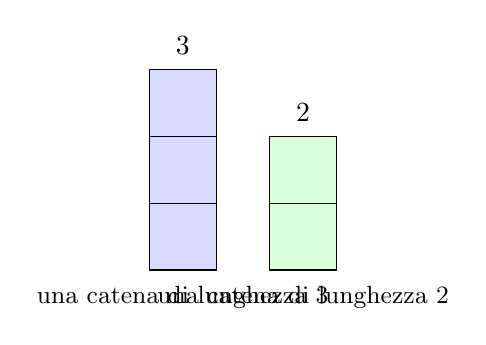
\begin{tikzpicture}[scale=0.85]
    % blocco da 3
    \draw[fill=blue!15] (0,0) rectangle (1,1);
    \draw[fill=blue!15] (0,1) rectangle (1,2);
    \draw[fill=blue!15] (0,2) rectangle (1,3);

    % blocco da 2
    \draw[fill=green!15] (1.8,0) rectangle (2.8,1);
    \draw[fill=green!15] (1.8,1) rectangle (2.8,2);

    \node at (0.5,3.35) {$3$};
    \node at (2.3,2.35) {$2$};

    \node at (0.5,-0.4) {\small una catena di lunghezza $3$};
    \node at (2.3,-0.4) {\small una catena di lunghezza $2$};
\end{tikzpicture}
\caption{Lettura delle lunghezze delle catene dai valori $\mu_1=2$, $\mu_2=4$, $\mu_3=5$.}
\end{figure}

\subsection{Andamento temporale associato}

Nel continuo, poiché $\lambda=0$, si ha
\[
e^{J_0^{(2)}t}
=
\begin{pmatrix}
1 & t\\
0 & 1
\end{pmatrix},
\qquad
e^{J_0^{(3)}t}
=
\begin{pmatrix}
1 & t & \dfrac{t^2}{2}\\
0 & 1 & t\\
0 & 0 & 1
\end{pmatrix}.
\]

Dunque
\[
e^{Jt}
=
\begin{pmatrix}
1 & t & 0 & 0 & 0\\
0 & 1 & 0 & 0 & 0\\
0 & 0 & 1 & t & \dfrac{t^2}{2}\\
0 & 0 & 0 & 1 & t\\
0 & 0 & 0 & 0 & 1
\end{pmatrix}.
\]

I modi presenti sono quindi del tipo:
\[
1,\qquad t,\qquad t^2.
\]

\paragraph{Interpretazione.}
Questo è un punto molto importante:
\begin{itemize}
    \item il modo costante $1$ corrisponde a una componente che non decade;
    \item il termine $t$ introduce crescita polinomiale;
    \item il termine $t^2$ introduce una crescita ancora più forte.
\end{itemize}

Quindi il sistema non è asintoticamente stabile.

\section{I modi del sistema e il ruolo dei blocchi di Jordan}

Possiamo ora formulare con precisione il messaggio strutturale della lezione.

\subsection{Nel tempo continuo}

Se un blocco di Jordan reale di ordine $r$ è associato all'autovalore $\lambda$, allora i modi che compaiono sono:
\begin{equation}
e^{\lambda t},\quad
te^{\lambda t},\quad
t^2 e^{\lambda t},\quad
\dots,\quad
t^{r-1}e^{\lambda t}.
\label{eq:L8_modes_CT}
\end{equation}

\subsection{Nel tempo discreto}

In modo analogo, nel discreto compaiono andamenti del tipo
\begin{equation}
\lambda^k,\quad
k\lambda^k,\quad
k^2\lambda^k,\quad
\dots
\label{eq:L8_modes_DT}
\end{equation}
a meno di coefficienti costanti o equivalenze del tipo $\binom{k}{j}\lambda^{k-j}$.

\paragraph{Osservazione.}
Dal punto di vista qualitativo, ciò che conta è la presenza del fattore polinomiale in $t$ oppure in $k$.

\section{Quando i blocchi di Jordan diventano decisivi}

Per autovalori ``non critici'', il segno della parte reale (nel continuo) o il modulo (nel discreto) basta spesso a descrivere il comportamento asintotico.

Ma per autovalori \emph{critici} bisogna guardare il blocco di Jordan massimo associato.

\subsection{Tempo continuo}

Nel continuo, il caso critico è
\[
\Re(\lambda)=0.
\]

Infatti:
\begin{itemize}
    \item se $\Re(\lambda)<0$, anche eventuali fattori polinomiali vengono dominati dal decadimento esponenziale;
    \item se $\Re(\lambda)>0$, il sistema diverge comunque;
    \item se $\Re(\lambda)=0$, la presenza di blocchi di ordine superiore a $1$ introduce termini tipo $t$, $t^2$, \dots, e può far perdere la stabilità.
\end{itemize}

\subsection{Tempo discreto}

Nel discreto, il caso critico è
\[
|\lambda|=1.
\]

Infatti:
\begin{itemize}
    \item se $|\lambda|<1$, il sistema tende a zero;
    \item se $|\lambda|>1$, il sistema diverge;
    \item se $|\lambda|=1$, la presenza di blocchi di Jordan di ordine superiore a $1$ introduce fattori tipo $k$, $k^2$, \dots, e può rendere il sistema instabile.
\end{itemize}

\paragraph{Morale pratica.}
Per ogni autovalore critico bisogna sempre controllare la dimensione del blocco di Jordan più grande a esso associato.

\section{Osservazione conclusiva sul significato dei modi}

Quando si porta una matrice in forma di Jordan, non lo si fa per un gusto puramente algebrico, ma perché nella matrice esponenziale dei blocchi di Jordan si leggono direttamente i modi temporali del sistema.

In altre parole:
\[
A = QJQ^{-1}
\quad \Longrightarrow \quad
e^{At} = Qe^{Jt}Q^{-1}.
\]

La matrice $Q$ cambia coordinate, ma non cambia la natura degli andamenti.  
Gli andamenti elementari li troviamo in $e^{Jt}$.

Per questo, i modi del sistema dipendono da:
\begin{itemize}
    \item gli autovalori;
    \item il loro valore numerico;
    \item la loro molteplicità algebrica;
    \item la dimensione dei blocchi di Jordan associati.
\end{itemize}

\section{Sintesi finale della lezione}

In questa lezione abbiamo visto che:

\begin{enumerate}
    \item gli autovettori generalizzati di una stessa catena sono linearmente indipendenti;
    \item una catena di lunghezza $k$ genera un sottospazio ciclico $A$-invariante di dimensione $k$;
    \item i numeri
    \[
    \mu_j=\dim\ker(A-\lambda I)^j
    \quad\text{e}\quad
    n_j=\mu_j-\mu_{j-1}
    \]
    permettono di ricostruire la struttura dei blocchi di Jordan;
    \item un blocco di Jordan di ordine $r$ associato a $\lambda$ produce nel continuo modi del tipo
    \[
    e^{\lambda t},\ te^{\lambda t},\ \dots,\ t^{r-1}e^{\lambda t};
    \]
    \item nel discreto compaiono analogamente termini del tipo
    \[
    \lambda^k,\ k\lambda^k,\ k^2\lambda^k,\dots;
    \]
    \item nei casi critici, cioè $\Re(\lambda)=0$ nel continuo oppure $|\lambda|=1$ nel discreto, la dimensione del blocco di Jordan è decisiva per stabilire il comportamento del sistema.
\end{enumerate}

Questa è la vera ragione per cui si studia la forma di Jordan: essa rende leggibili, in modo immediato, i modi strutturali del sistema.